\section{Domain Name System}

    A utilização de um sistema de resolução de nomes permite que o \textit{tracker} conheça o nome dos \textit{end systems} em vez dos seus endereços IP, como tal é essencial realizar algumas alterações no segmento \textit{TCPPacket}, nomeadamente acrescentar um campo \textit{hostname}.

    Durante as aulas práticas foi mencionado que deveríamos usufruir de uma solução que tivesse por base \textit{bind}, algo que estudamos durante imenso tempo e tentámos implementar.

    Infelizmente desistimos desse caminho, pois nenhum docente forneceu-nos qualquer base sobre como utilizar o serviço \textit{bind9} na topologia do \textit{CORE}, e quando descobrimos já era tarde de mais para poder voltar atrás.

    Assim sendo, fomos obrigados a implementar um protocolo de DNS e o seu respetivo servidor, percebemos que seria importante haver uma redundância de servidores DNS, contudo o tempo urge e não nos permite qualquer margem de manobra.

    Em termos práticos, um servidor DNS possui um \textit{map} no qual associa \textit{hostnames} a endereços IP, como tal o cabeçalho dos segmentos utilizados para resolver um determinado nome é bastante simplista.

    \newpage
    \begin{figure}[hb!]
        \centering
        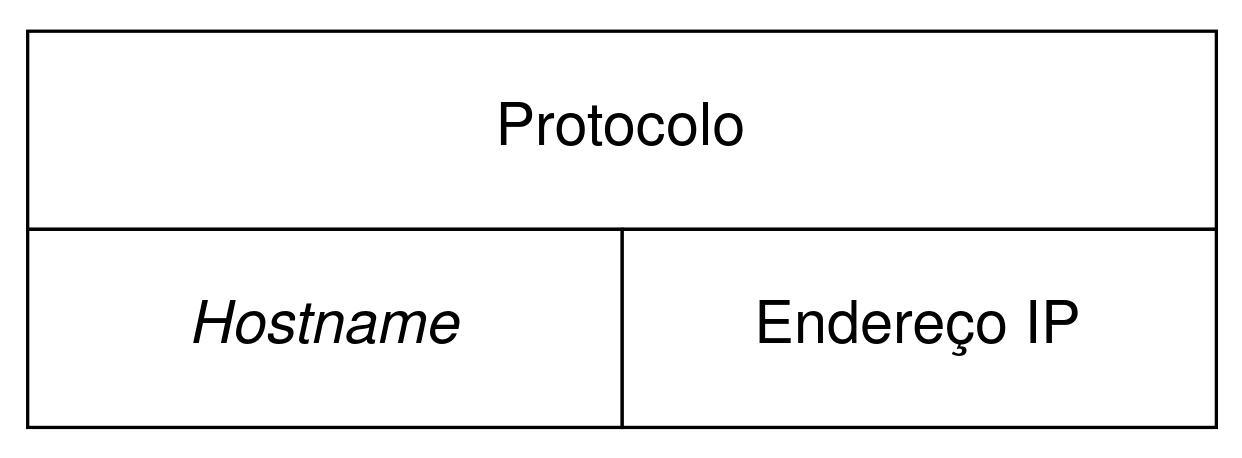
\includegraphics[width=0.45\textwidth]{Imagens/Headers/dns.png}
        \caption{Cabeçalho de um \textit{DNSPacket}}
    \end{figure}

    O campo \textit{Protocolo} pode parecer um pouco inútil, visto que o único objetivo deste serviço é resolver um determinado nome, todavia torna-se crucial nos momentos em que é necessário avisar o servidor DNS do aparecimento/desaparecimentos de nós.

    Originalmente o DNS usufrui do UDP como forma de maximizar a velocidade do serviço, todavia optámos por utilizar TCP, visto que isso facilita bastante a implementação do código.

    \begin{figure}
        \centering
        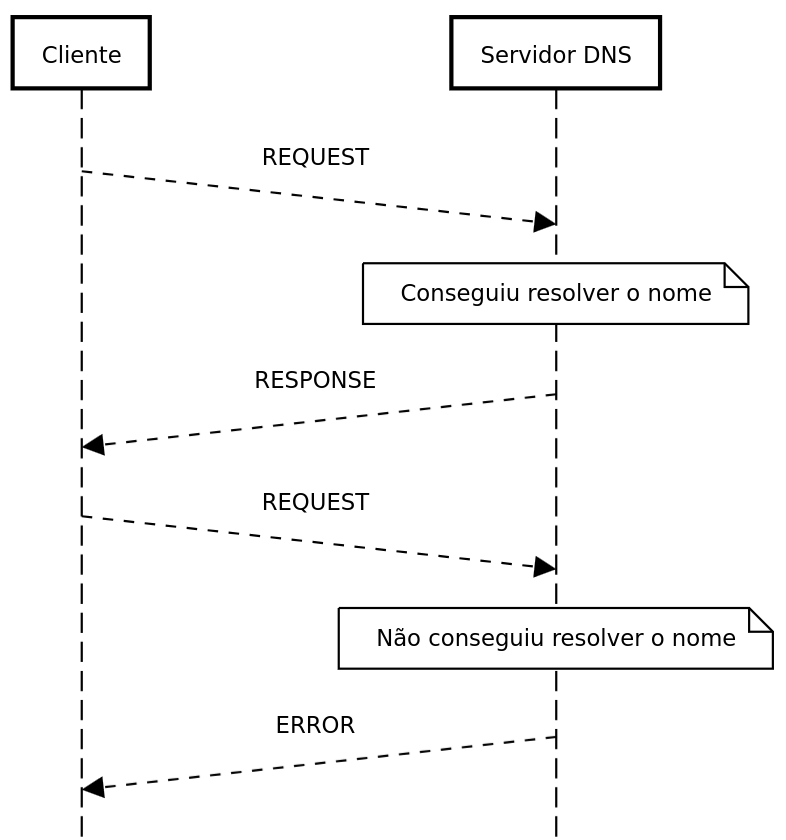
\includegraphics[width=0.47\textwidth]{Imagens/Diagramas Temporais/dns.png}
        \caption{Diagrama temporal da resolução de nomes}
    \end{figure}

    \begin{enumerate}
        
        \item O cliente pretende obter o endereço IP associado a um \textit{hostname}.

        \item É enviado um \textit{REQUEST} ao servidor DNS.

        \item O servidor DNS verifica se o \textit{hostname} recebido existe na sua estrutura de dados.

        \item Em caso afirmativo é envidado um \textit{RESPONSE} com o endereço IP, caso contrário é transmitido um \textit{ERROR}.

    \end{enumerate}